\chapter{极限精度梯度压缩方法}
考虑到梯度数据普遍较小,绝大部分数据绝对值在0~1之间的特点,如表~\ref{tab:resnet50_1iter_grad_fabs}所示。在Resnet50网络中,每次迭代需要更新155个tensor的梯度,表中展示了在第一次迭代中各个tensor最大绝对值所处的范围。可知仅考虑每个tensor中最大绝对值情况下,53.55\%的tensor中最大绝对值在0~1之间;41.29\%的tensor中最大绝对值在1~10之间;仅有5.16\%的tensor中最大绝对值在10~50之间。
\begin{table}[htb]
\centering
\noindent\begin{minipage}{0.65\textwidth}
\centering
\caption{Resnet50第一次迭代中各层梯度最大绝对值分布}
\label{tab:resnet50_1iter_grad_fabs}
\begin{tabular}{p{2.5cm}p{2.5cm}p{2.5cm}}
\toprule[1.5pt]
梯度绝对值 & 数量 & 占比(\%) \\\midrule[1pt]
0~1.0 & 83 & 53.55\\
1.0~10.0 & 64 & 41.29\\
10.0~50.0 & 8 & 5.16\\
\midrule[1pt]
\end{tabular}
\end{minipage}
\end{table}

随着训练的进行,网络逐渐趋向于稳定,梯度数据的波动范围更小,更集中于0~1之间。如表~\ref{tab:resnet50_21iter_grad_fabs}所示。在第21次迭代中绝对值在0~1之间的梯度占比为74.84\%,1~10和10~50之间的梯度数量相对减少。可知在后面训练的迭代中梯度数据的绝对值将更加集中于0~1之间。故本章希望针对梯度数据这一特点,使用更少比特位表示梯度。通过减少梯度数据的表示位,可减少分布式训练过程中的同步数据量,进而提高分布式系统的可扩展性和训练效率。
\begin{table}[htb]
\centering
\noindent\begin{minipage}{0.65\textwidth}
\centering
\caption{Resnet50第21次迭代中各层梯度最大绝对值分布}
\label{tab:resnet50_21iter_grad_fabs}
\begin{tabular}{p{2.5cm}p{2.5cm}p{2.5cm}}
\toprule[1.5pt]
梯度绝对值 & 数量 & 占比(\%) \\\midrule[1pt]
0~1.0 & 116 & 74.84\\
1.0~10.0 & 37 & 23.87\\
10.0~50.0 & 2 & 1.29\\
\midrule[1pt]
\end{tabular}
\end{minipage}
\end{table}

本章希望在不影响神经网络训练精度的情况下,尽可能减少梯度数据所需的比特位数,为进一步减少分布式通信开销,提高分布式系统可扩展性和训练效率提供数据压缩方法。本章将主要介绍梯度压缩的思路与实现方法,以及对应压缩方式在图像分类和物体检测网络中的训练精度。通过其与原始的训练精度对比,说明对应压缩算法的有效性和适用范围。本章针对图像分类、物体检测任务分别提出三种极限精度梯度压缩EPGC方法。图像分类任务对梯度数据精度要求低,本文提出9比特梯度压缩方法和8比特梯度压缩方法;考虑到物体检测网络对梯度数据精度要求偏高,具体原因将在后面详细分析,本文提出11比特梯度压缩方法。经实验证明:本文提出的三种极限精度梯度压缩EPGC方法,在图像分类或物体检测任务中均能达到原始训练相同收敛精度。说明了这三种梯度压缩方法在各自任务中的有效性,以及通过该压缩方法在保证神经网络收敛精度前提下,提升分布式系统可扩展性和训练效率的可行性。
\section{引言}
根据第二章内容可知,分布式训练过程中同步开销的大小对系统的可扩展性和训练效率有至关重要的影响。在不影响训练精度的情况下,将梯度尽可能地压缩则可减少同步开销,提高分布式系统的可扩展性和训练效率。本章将分别介绍适用于图像分类和物体检测网络的不同梯度压缩方法,将详细分析其具体实现和各个压缩方式下分类网和物体检测网络的最终收敛精度。

由第三章LPDU算法实现可知,基于horovod要实现新的数据压缩方法,则需在MPI中新增一个数据类型来解析该压缩数据,并实现一个该数据类型的求和函数供MPI调用。为快速验证本文针对图像分类和物体检测任务分别提出的梯度压缩方法对网络训练精度的影响,本章提出的梯度压缩方法均通过对FP32浮点数或半精度浮点数对应比特位清零的方式来模拟对应的压缩方法。该模拟方法可避免对MPI的改动,使得本章提出的压缩方法能够快速得到验证。下面将对适用于图像分类网络的两种EPGC方法:9比特梯度压缩方法和8比特梯度压缩方法;以及适用于物体检测网络的10比特梯度压缩方法进行详细介绍。
\section{分类网络中的梯度压缩方法}
本节主要介绍适用于图像分类网络的两种梯度压缩方法:9比特梯度压缩方法和8比特梯度压缩方法。实验证明这两种压缩方法在分类网络中均能达到理想收敛精度,但在性能上各有优缺点。

9比特梯度压缩方法核心思路是:在浮点数基础上,去除所有尾数比特位,仅保留1位符号位,8位指数位来表示梯度。在实现过程中浮点数与9比特数据格式的转换可以高效完成;而8比特梯度压缩方法核心思路是:将浮点数梯度转换为16比特的半精度数据,再在FP16数据基础上去除8位尾数位,仅使用8比特(1位符号位,5位指数位,2位尾数位)表示梯度。从其压缩思路可知,在实现过程中需要完成浮点数到半精度数据的转换和半精度数据到8比特数据的转换,其开销稍大于9比特梯度压缩方法。但该压缩方法所需传输的数据量少于90比特梯度压缩方法;其在半精度训练场景中,该方法能够更为高效实现。
\subsection{9比特梯度压缩方法}
根据上一章LPDU算法可知,BF16数据格式相对于原始FP32数据而言,去除了浮点数尾数中的后16比特位,仅保留7位有效比特位。本压缩算法根据这一思路,在BF16数据基础上,进一步减少尾数有效位,在保证训练精度情况下,尽可能减少尾数比特位,以减少分布式同步中的数据通信量。
\begin{figure}[htp]
\centering
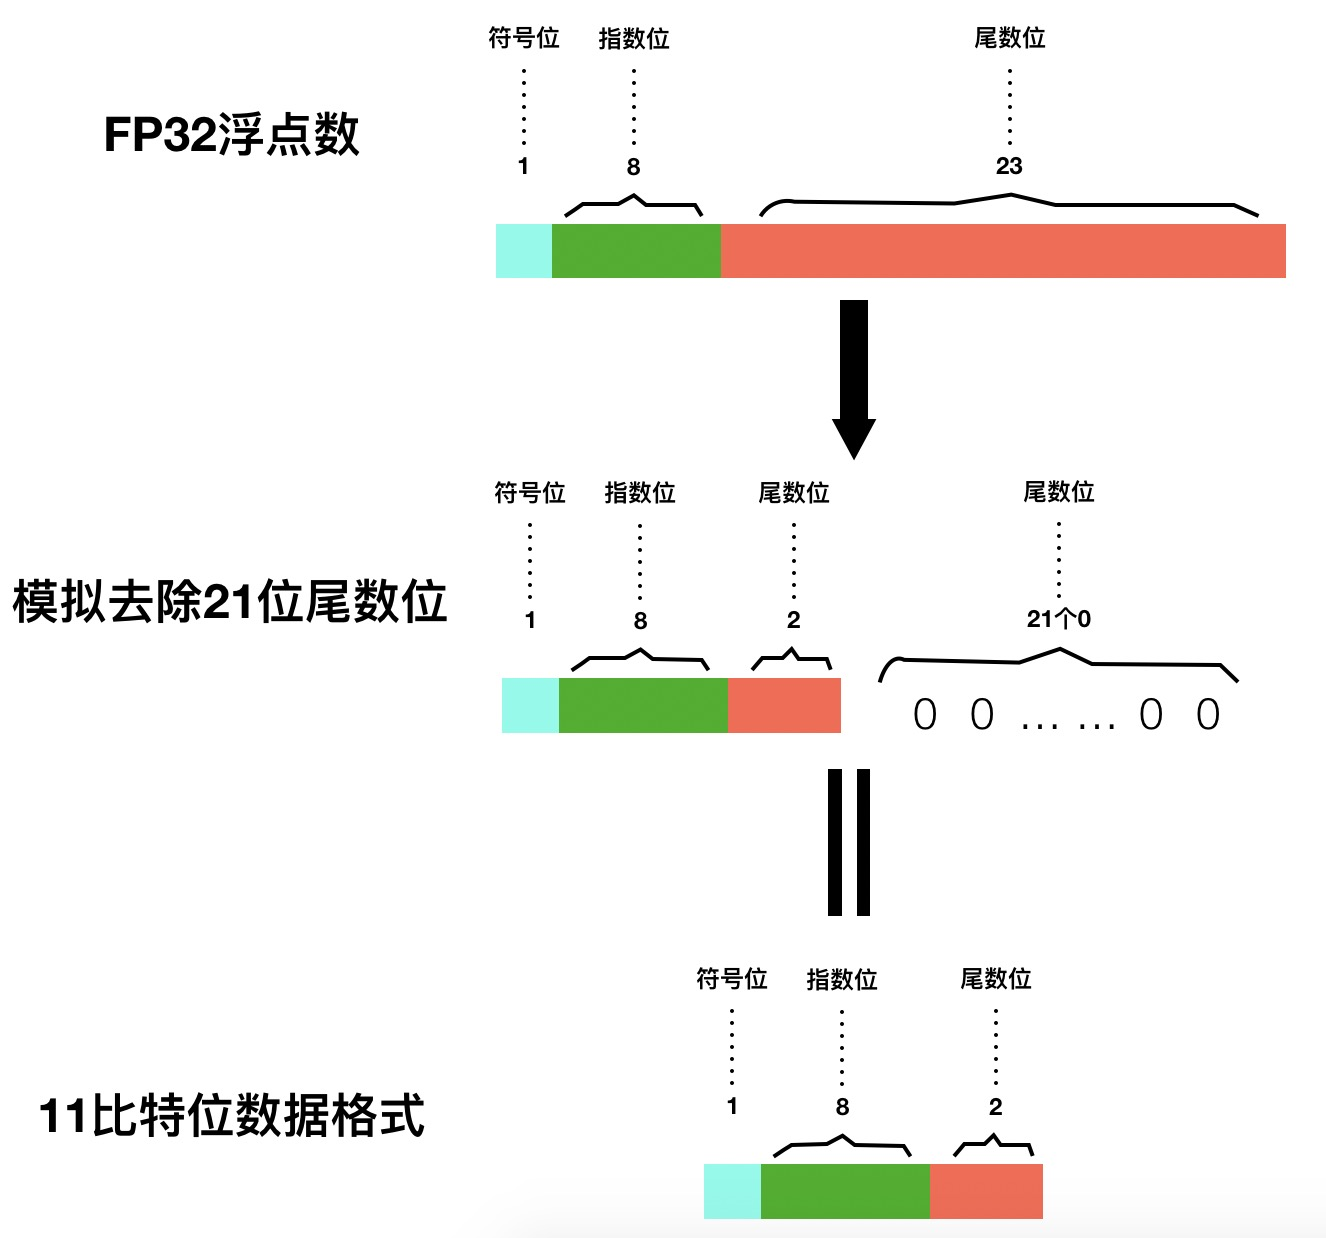
\includegraphics[width=10cm]{simulate_11bits}
\caption{模拟11比特数据表示示意图}
\label{fig:simulate_11bits}
\end{figure}

本节通过对原始FP32浮点数尾数位清零的方法模拟这种压缩方法。如在FP32浮点数基础上仅保留两位有效尾数位,形成11比特的数据格式,可通过将FP32浮点数的低21位清零达到相同效果,如图~\ref{fig:simulate_11bits}所示。可知低21比特位清零后的浮点数等效于11比特位数据格式所表示数据。

使用这种模拟方法,本文逐渐减少尾数比特位,并使用对应梯度压缩方法训练图像分类领域经典网络Resnet50,来验证该压缩方法在图像分类任务中的有效性。最终发现在去除所有尾数情况下,仅使用9比特梯度压缩算法即可保证分类网的训练精度,故本节提出了适用于图像分类网络的9比特梯度压缩方法。

\subsection{9比特梯度压缩方法实验分析}
通过这种模拟方法,本文分别得出使用11比特,10比特,9比特情况下,压缩算法对分类网的影响,以Resnet50为例。经实验验证:在同步梯度数据时仅保留两比特位的尾数情况下,分类网也可收敛到原始浮点数梯度相同精度。在11比特有效位基础上,继续减少尾数位,保留1位尾数、去除所有尾数位情况下,在分类网上均能达到理想收敛精度。在去除所有尾数位仅使用9比特数据表示梯度情况下,Resnet50的收敛曲线如图~\ref{fig:simulate_9bits_acc}所示。

\begin{figure}[htp]
\centering
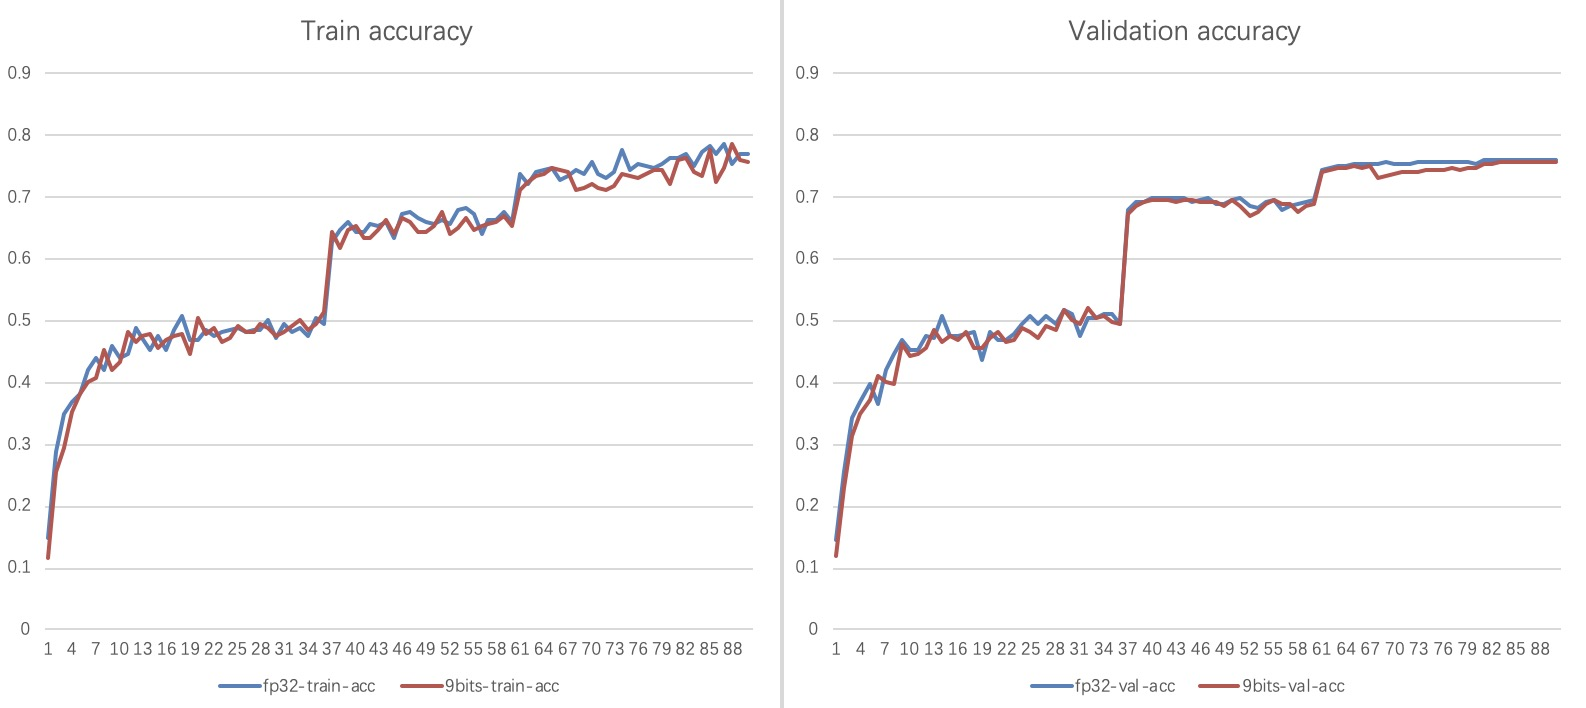
\includegraphics[width=13cm]{simulate_9bits_acc2}
\caption{9比特梯度压缩方法与原始浮点数表示下Resnet50训练精度曲线}
\label{fig:simulate_9bits_acc}
\end{figure}

保留2位尾数,1位尾数,不保留尾数情况下,Resnet50在验证集准确率如表~\ref{tab:simulate_11_10_9bits_acc}所示。所有结果均在4节点8实例配置下训练得到。由表~\ref{tab:simulate_11_10_9bits_acc}可知,在原始浮点梯度基础上,仅保留2位尾数,1位尾数,不保留尾数情况下,Resnet50网络精度与原始浮点数梯度精度相差<0.3\%。说明在误差允许范围内,在分类网中仅使用9比特数据(1个符号位,8个指数位)表示梯度即可满足分类网的训练精度要求。通过去除浮点数中所有尾数位的方法可在不影响神经网络训练精度前提下减少分布式同步开销,提升分布式系统的可扩展性和训练效率。

\begin{table}[htb]
\centering
\noindent\begin{minipage}{0.6\textwidth}
\centering
\caption{不同尾数位下Resnet50准确率}
\label{tab:simulate_11_10_9bits_acc}
\begin{tabular}{p{2cm}p{2.5cm}}
\toprule[1.5pt]
有效尾数位 & Resnet50 acc(\%) \\\midrule[1pt]
FP32 & 76.12 \\
2 & 76.08 \\
1 & 76.01 \\
0 & 75.87 \\
\midrule[1pt]
\end{tabular}
\end{minipage}
\end{table}

\subsection{8比特梯度压缩方法}
由本文第二章可知,半精度浮点数也可用于训练神经网络,也能保证网络的训练精度与原始浮点数训练一致。半精度浮点数与BF16数据格式相比,少了3个指数位,仅5个指数位。根据上一节9比特梯度压缩方法可知,在仅保留2位,1位尾数或不保留尾数位情况下,均能保证图像分类网络训练精度与原始浮点数训练精度在误差允许范围内。本节结合半精度浮点数特点,提出8比特梯度压缩方法:在半精度浮点数基础上,去除16位半精度浮点数中低8位尾数,仅保留两个有效尾数位,使用8比特数据表示梯度,以此将梯度压缩成单字节数据。由前文可知:该方法相对于9比特梯度压缩方法而言,在使用浮点数训练情况下其实现开销较大;但其通信开销较小,且在半精度浮点数训练模型下,8比特梯度压缩方法能够更高效的实现。

为快速验证本节所提出的梯度压缩方法的有效性,本节通过将半精度浮点数特定尾数位清零的方式模拟该压缩方法。原理如图~\ref{fig:simulate_8bits}所示。可知将FP16格式数据低8比特位清零后的半精度浮点数等效于8比特位数据格式所表示数据。

\begin{figure}[htp]
\centering
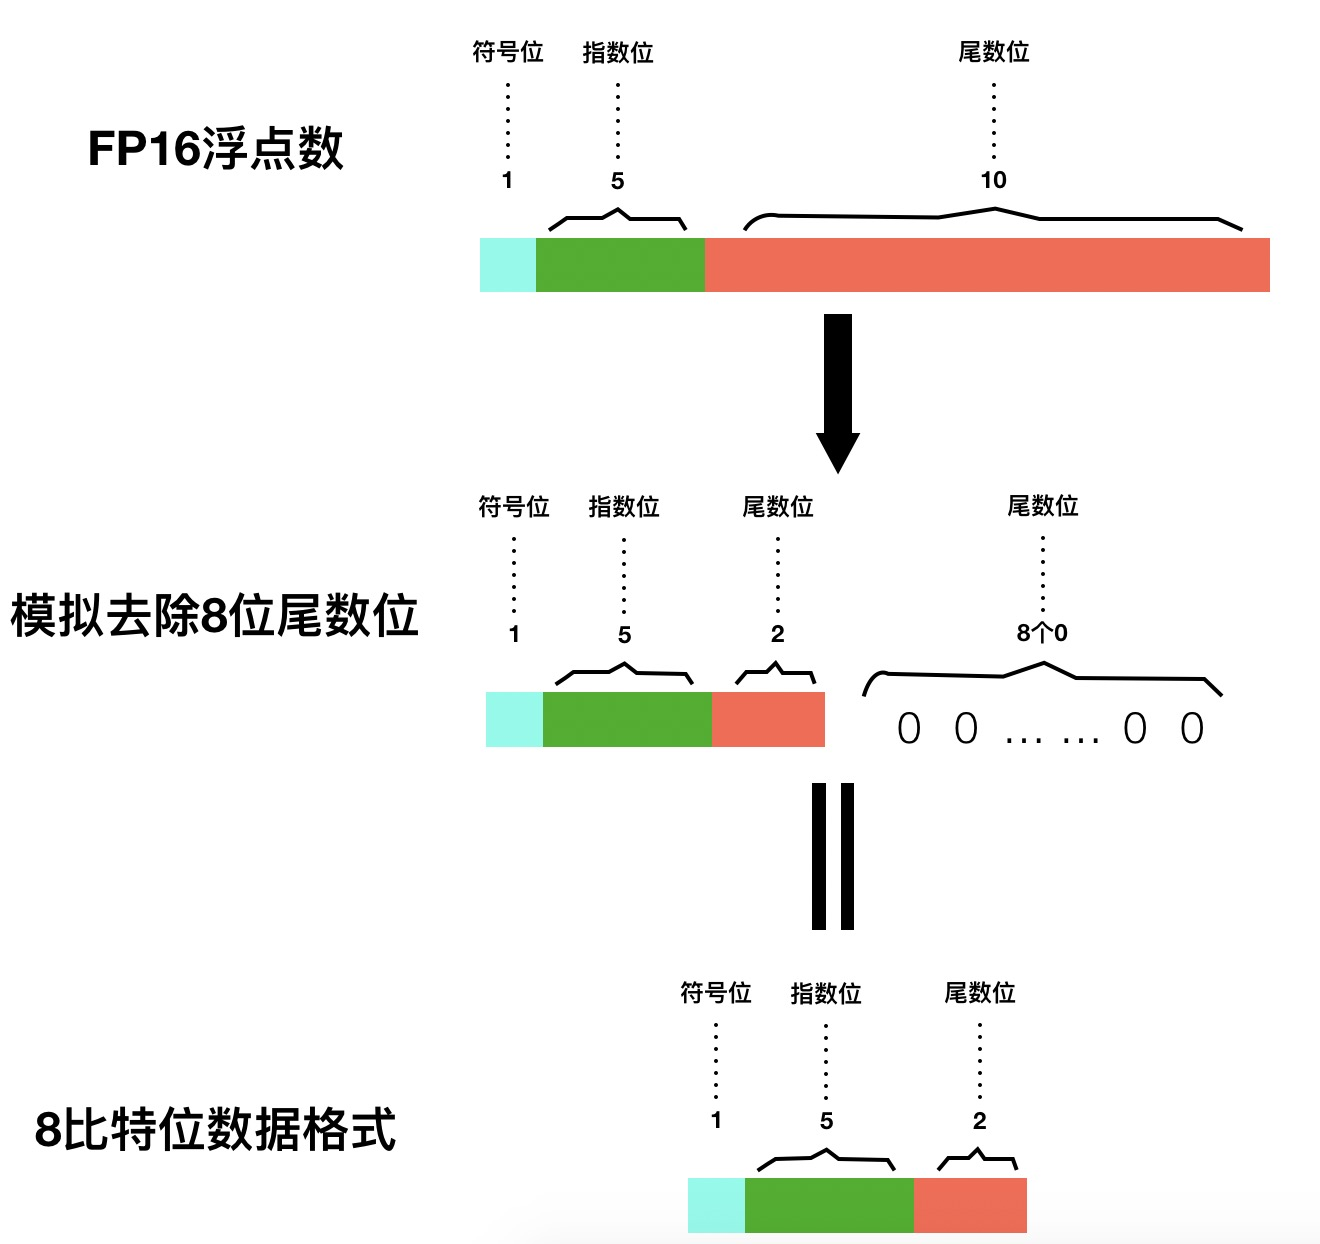
\includegraphics[width=10cm]{simulate_8bits}
\caption{模拟8比特数据表示示意图}
\label{fig:simulate_8bits}
\end{figure}

本文在Resnet50训练中使用这种8比特梯度压缩方法,通过比较网络与原始浮点数训练的收敛精度来验证该梯度压缩方法的有效性和适用范围。实验发现本节提出的8比特梯度压缩方法在分类网训练中不会对网络精度造成影响。

在该8比特梯度压缩方法下,神经网络训练流程如图~\ref{fig:8bits_workflow}所示。整个训练流程类似于第三章LPDU算法下的训练流程。但8比特梯度压缩方法的数据转换过程较为复杂。首先需要将浮点数转换成半精度浮点数,该过程涉及到数据位的转换,比较耗时;再在半精度浮点数基础上去除8比特尾数位,仅使用8比特梯度数据进行通信。完成8比特的数据通信后,通过8比特数据到半精度浮点数,半精度浮点数到浮点数的转化,将8比特数据恢复成浮点数。当使用半精度浮点数训练神经网络时,8比特梯度压缩方法的训练流程则可直接去除浮点数与半精度数据的转化过程,在这种情况下8比特梯度压缩方法最为高效。
\begin{figure}[htp]
\centering
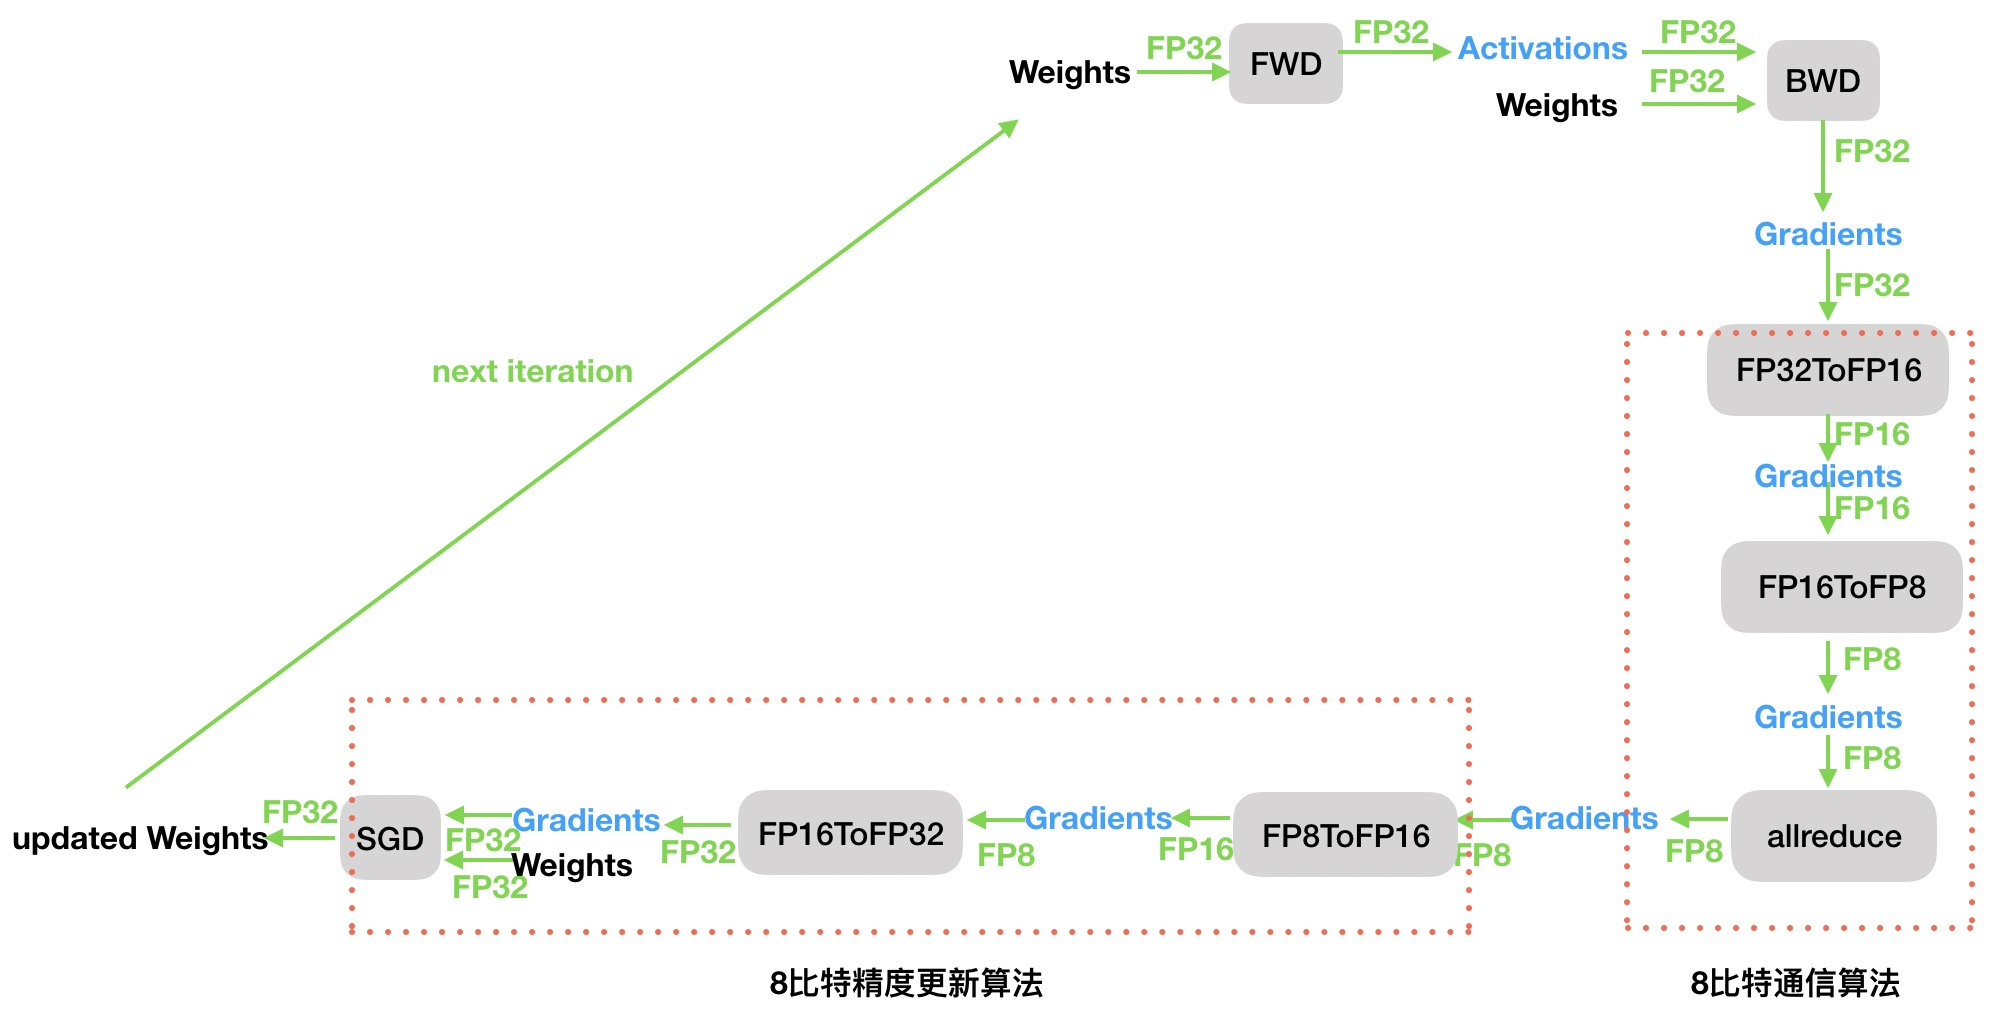
\includegraphics[width=10cm]{8bits_workflow}
\caption{8比特梯度压缩方法下训练流程图}
\label{fig:8bits_workflow}
\end{figure}

\subsection{8比特梯度压缩方法实验分析}
在4节点8实例情况下,使用该方法将梯度数据压缩成单字节数据,Resnet50的收敛曲线如图~\ref{fig:simulate_8bits_acc}所示。可知本节提出的8比特梯度压缩方法同样能达到原始训练精度:76.1\%,说明本节提出的压缩方法可在不影响分类网络精度情况下,减小分布式训练神经网络中的通信量,从而提升分布式系统的可扩展性和训练效率。
\begin{figure}[htp]
\centering
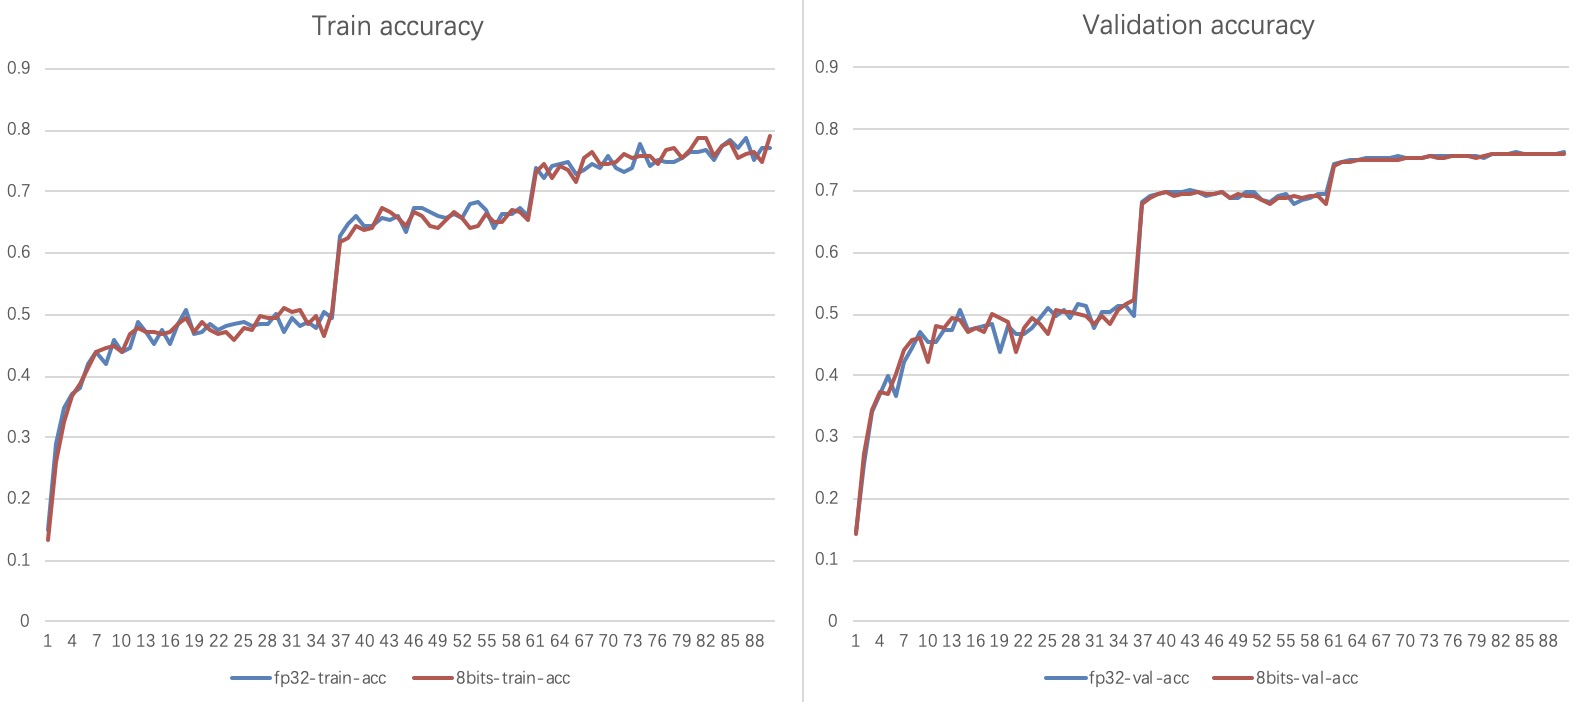
\includegraphics[width=13cm]{simulate_8bits_acc2}
\caption{8比特位梯度压缩方法与原始浮点数表示下Resnet50精度曲线}
\label{fig:simulate_8bits_acc}
\end{figure}

根据上一节提出的9比特压缩方法可知,可进一步在半精度浮点数上减少尾数位或去除所有尾数位,极限情况下仅使用6比特数据表示梯度。下一步将对这种可能的6比特梯度压缩方法在分类网络中进行尝试验证,通过比较该梯度压缩方法下分类网的最终收敛精度与原始收敛精度的差异,说明该梯度压缩算法对分类网精度的影响,从而确定该梯度压缩算法应用于分类网络的可行性。

\section{物体检测网络中的梯度压缩方法}
\subsection{物体检测网络精度要求分析}
在目前一阶段、二阶段的物体检测网络中,均是把物体检测任务当成多任务来处理。主要包含:分类任务和回归任务。回归任务目的是通过逻辑回归的方式得到物体的坐标位置,即$(x,y,w,h)$。$x,y$表示物体框的中心坐标,$w,h$则表示物体框的宽和高。分类任务则是判断对应物体框的类别,与分类网类似。这两个任务共同完成物体检测任务。回归任务中关于$(x,y,w,h)$的计算如公式~\ref{equ:regression_equ}所示。$t(x,y,w,h)$表示对应输出特征图的值,$P(x,y,w,h)$表示原始anchor对应的坐标信息。根据特征图信息和对应anchor的坐标信息进行计算得出的坐标即为网络预测物体的坐标。

\begin{equation}
\label{equ:regression_equ}
\begin{split}
\hat{G_{x}} &=P_{w}t_{x}+P_{x} \\
\hat{G_{y}} &=P_{h}t_{y}+P_{y} \\
\hat{G_{w}} &=P_{w}e^{t_{w}} \\
\hat{G_{h}} &=P_{h}e^{t_{h}} 
\end{split}
\end{equation}

由公式~\ref{equ:regression_equ}可知,$\hat{G_{w}}, \hat{G_{h}}$的计算过程中需要将网络输出的值求$e$的指数,再乘上anchor的长或宽。根据指数函数$e^{x}$导数性质可知,$x$的较小变化,将可能对指数结果$e^{x}$造成巨大差异。故当梯度数据精度过低导致对应输出特征图与原始浮点数更新下的特征图的稍小差异,可能在指数函数作用下产生数倍数量级的差距。从而造成检测网络精度无法达到理想收敛精度。如在保留2位尾数,1位尾数,去除所有尾数以及8比特梯度压缩方法下SSD网络的收敛曲线如图~\ref{fig:low_bits_ssd}所示。
\begin{figure}[htp]
\centering
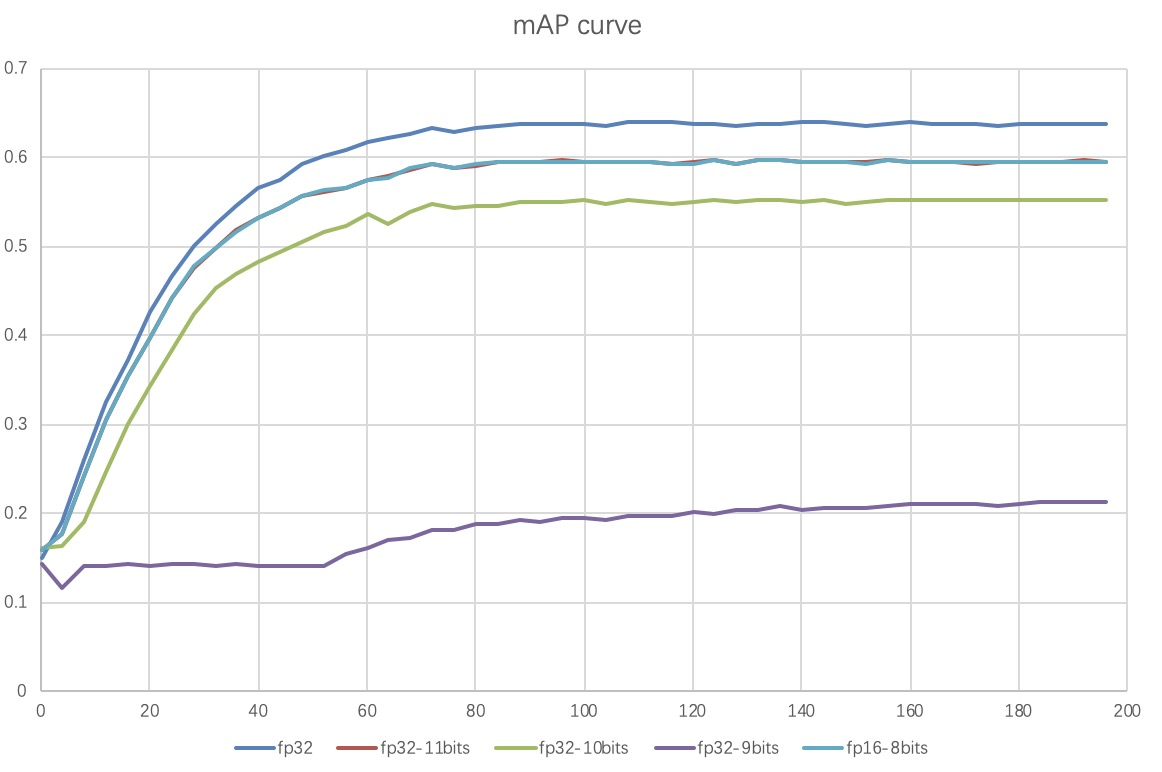
\includegraphics[width=12cm]{low_bits_ssd}
\caption{SSD在不同比特压缩算法下mAP曲线}
\label{fig:low_bits_ssd}
\end{figure}

由图~\ref{fig:low_bits_ssd}所示,在仅保留2比特尾数情况下,SSD最终收敛的mAP指略低于原始浮点数训练的收敛精度。随着尾数位的降低,其收敛精度也逐渐降低;可以看出:8比特梯度压缩方法下收敛曲线与基于浮点数的11比特梯度压缩方法的曲线基本重合,其原因在于这两种梯度压缩方法的尾数位均相同,因为梯度数据本身数值范围较小,指数位的减小不会对网络精度造成影响。图~\ref{fig:low_bits_ssd}充分说明了物体检测网络因为存在回归坐标任务的存在,使得其对梯度数据的精度要求高于分类网络,适用于分类网络的极限梯度压缩EPGC方法不能保证物体检测网络的训练精度。不同梯度压缩方法下SSD最终收敛精度如表~\ref{tab:ssd_accs}所示。
\begin{table}[htb]
\centering
\noindent\begin{minipage}{0.6\textwidth}
\centering
\caption{不同梯度压缩方法下SSD最终mAP}
\label{tab:ssd_accs}
\begin{tabular}{p{2cm}p{2cm}p{2.5cm}}
\toprule[1.5pt]
有效位数 & 有效尾数位 & SSD mAP(\%) \\\midrule[1pt]
32 & 23 & 64.00 \\
11 & 2 & 59.66 \\
10 & 1 & 55.33 \\
9 & 0 & 21.36 \\
8 & 2 & 59.78 \\
\midrule[1pt]
\end{tabular}
\end{minipage}
\end{table}

\subsection{11比特梯度压缩方法与实验}
由上一节分析可得出两个结论:1.物体检测网络对梯度数据精度要求高于分类网络;2.将梯度数据指数位由8比特减少至5比特不会对神经网络训练精度造成影响。基于这两点认识,本节希望在8比特梯度压缩方法基础上,逐渐增加梯度数据尾数位,并在对应尾数位下训练物体检测网络,通过比较其最终收敛精度是否达到原始浮点数训练的收敛精度来验证该种梯度压缩方法在物体检测网络中的有效性。

同理,为快速验证本节提出的梯度压缩方法的有效性,所有梯度压缩方法均通过在半精度浮点数基础上对特定尾数位清零的方式模拟所得。原理与图~\ref{fig:simulate_8bits}类似。

通过该模拟方法,本节分别得出使用9比特,10比特,11比特情况下,对应梯度压缩方法对物体检测网络收敛精度的影响。经实验验证:保留5位尾数位,使用11比特梯度压缩方法能保证物体检测网络的收敛精度。9比特,10比特,11比特梯度压缩方法下物体检测网络的mAP曲线如图~\ref{fig:ssd_epgc_accs}所示。可知,随着梯度数据尾数位的逐渐增加,物体检测网络的训练曲线越来越接近于原始浮点数的训练曲线。当尾数比特位增加至5位时,11比特梯度压缩方法下SSD的收敛曲线基本与原始浮点数训练的收敛曲线重合,说明了11比特梯度压缩方法不会对物体检测网络训练精度造成影响。验证了11比特梯度压缩方法通过减少通信数据量,提高分布式系统的可扩展性和训练效率的可行性。9比特,10比特,11比特梯度压缩方法下SSD最终收敛精度如表~\ref{tab:ssd_epdc_final_accs}所示。

\begin{figure}[htp]
\centering
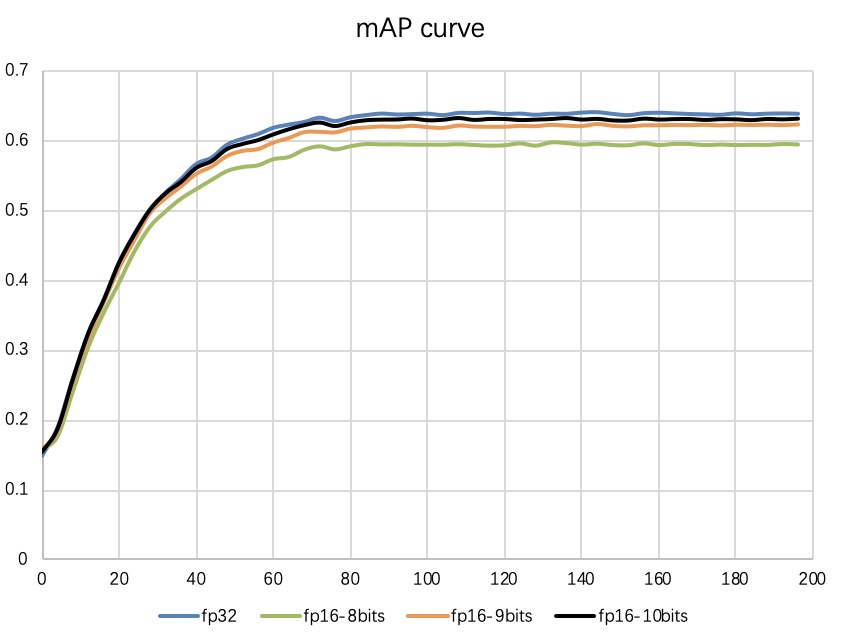
\includegraphics[width=12cm]{ssd_epgc_accs}
\caption{不同梯度压缩方法下SSD mAP曲线}
\label{fig:ssd_epgc_accs}
\end{figure}

\begin{table}[htb]
\centering
\noindent\begin{minipage}{0.6\textwidth}
\centering
\caption{8~11梯度压缩方法下SSD最终mAP}
\label{tab:ssd_epdc_final_accs}
\begin{tabular}{p{2cm}p{2cm}p{2.5cm}}
\toprule[1.5pt]
有效位数 & 有效尾数位 & SSD mAP(\%) \\\midrule[1pt]
32 & 23 & 64.00 \\
11 & 5 &  \\
10 & 4 & 63.24 \\
9 & 3 & 62.37 \\
8 & 2 & 59.78 \\
\midrule[1pt]
\end{tabular}
\end{minipage}
\end{table}

基于半精度浮点数不同比特位数的梯度压缩方法中,不同尾数位下数据精度信息如表~\ref{tab:ssd_epdc_precisions}所示。说明物体检测网络训练过程中,必须保证0.03125的数据精度才可保证网络的收敛精度与原始浮点数收敛精度保持一致。

\begin{table}[htb]
\centering
\noindent\begin{minipage}{0.5\textwidth}
\centering
\caption{不同尾数情况下数据精度}
\label{tab:ssd_epdc_precisions}
\begin{tabular}{p{2cm}p{2cm}p{2cm}}
\toprule[1.5pt]
有效位数 & 尾数位 & 数据精度 \\\midrule[1pt]
8 & 2 & 0.25000 \\
9 & 3 & 0.12500 \\
10 & 4 & 0.06250 \\
11 & 5 & 0.03125 \\
\midrule[1pt]
\end{tabular}
\end{minipage}
\end{table}

根据本节对物体检测网络对梯度数据精度要求偏高的原因以及相关实验结果,说明本节提出的适用于物体检测网络的11比特梯度压缩方法在不影响网络收敛精度的前提下,通过减少同步过程中数据通信量的方式提高分布式系统的可扩展性和训练效率的可行性。

\section{本章小结}

本章基于减少分布式训练神经网络通信开销,提高分布式系统的可扩展性和训练效率的目的,希望通过减少梯度数据比特位的方法来减少通信数据量。针对图像分类与物体检测任务对梯度数据精度要求不同,本章分别提出适用于图像分类任务的9比特,8比特梯度压缩方法和适用于物体检测任务的11比特梯度压缩方法。经实验验证针对于图像分类网络的两种极限梯度压缩EPGC方法:9比特梯度压缩方法和8比特梯度压缩方法在Resnet50网络中均能达到训练精度要求,说明将这两种梯度压缩方法应用于分类网络的可行性。从理论上分析了物体检测网络对梯度数据精度要求偏高的原因,并提出适用于物体检测网络的11比特梯度压缩方法,经实验验证11比特梯度压缩方法可保证物体检测网络训练精度与原始浮点数训练精度相同,说明了该压缩方法应用于物体检测网络训练的可行性。

下一步主要有两方面工作:1.基于8比特梯度压缩方法,继续减少尾数位,极限情况下仅使用6比特数据传输梯度,将其应用于分类网的训练,通过比较其训练精度与原始训练精度的差异,验证这种梯度压缩算法的可行性;2.针对分类网与物体检测网络对梯度数据精度要求不同的特点,本文分别提出了适用于分类网和物体检测网的极限梯度压缩EPGC方法。基于这一思路,本文希望将传统压缩算法引入到分布式同步通信中,根据不同任务的神经网络对梯度数据精度的不同要求,对传统压缩算法进行优化改进,使得在对应任务上达到更优的效果。



